\documentclass[11pt,a4paper]{article}
\usepackage[BoldFont,SlantFont,CJKchecksingle]{xeCJK}
\usepackage{fontspec}
\setmainfont{Courier New}
\usepackage{fontspec}
\setCJKmainfont{WenQuanYi Micro Hei}
\usepackage{xunicode}
\usepackage{xltxtra}
\usepackage{indentfirst}
\XeTeXlinebreaklocale “zh”
\XeTeXlinebreakskip = 0pt plus 1pt minus 0.1pt

\usepackage{ifxetex,ifluatex}
\ifxetex
  \usepackage{fontspec,xltxtra,xunicode}
  \defaultfontfeatures{Mapping=tex-text,Scale=MatchLowercase}
\else
  \ifluatex
    \usepackage{fontspec}
    \defaultfontfeatures{Mapping=tex-text,Scale=MatchLowercase}
  \else
    \usepackage[utf8]{inputenc}
  \fi
\fi
\usepackage{graphicx}
% We will generate all images so they have a width \maxwidth. This means
% that they will get their normal width if they fit onto the page, but
% are scaled down if they would overflow the margins.
\makeatletter
\def\maxwidth{\ifdim\Gin@nat@width>\linewidth\linewidth
\else\Gin@nat@width\fi}
\makeatother
\let\Oldincludegraphics\includegraphics
\renewcommand{\includegraphics}[1]{\Oldincludegraphics[width=\maxwidth]{#1}}
\ifxetex
  \usepackage[setpagesize=false, % page size defined by xetex
              unicode=false, % unicode breaks when used with xetex
              xetex,
              colorlinks=true,
              linkcolor=blue]{hyperref}
\else
  \usepackage[unicode=true,
              colorlinks=true,
              linkcolor=blue]{hyperref}
\fi
\hypersetup{breaklinks=true, pdfborder={0 0 0}}
\setlength{\parindent}{0pt}
\setlength{\parskip}{6pt plus 2pt minus 1pt}
\setlength{\emergencystretch}{3em}  % prevent overfull lines


\usepackage{framed,color}
\definecolor{shadecolor}{gray}{0.95}
\begin{document}

\section{Kmod 运行时调试图}

\subsection{编译安装运行调试图}

\subsubsection{wget下载源码包}

{\begin{shaded}\begin{verbatim}
$ wget https://www.kernel.org/pub/linux/utils/kernel/kmod/kmod-11.tar.gz
--2013-06-18 01:08:47--  https://www.kernel.org/pub/linux/utils/kernel/kmod/kmod-11.tar.gz
Resolving www.kernel.org (www.kernel.org)... 149.20.4.69, 198.145.20.140
Connecting to www.kernel.org (www.kernel.org)|149.20.4.69|:443... connected.
HTTP request sent, awaiting response... 200 OK
Length: 3458574 (3.3M) [application/x-gzip]
Saving to: `kmod-11.tar.gz'

100%[======================================>] 3,458,574    795K/s   in 5.3s    

2013-06-18 01:08:54 (641 KB/s) - `kmod-11.tar.gz' saved [3458574/3458574]
\end{verbatim}\end{shaded}}
\begin{figure}[htbp]
\centering
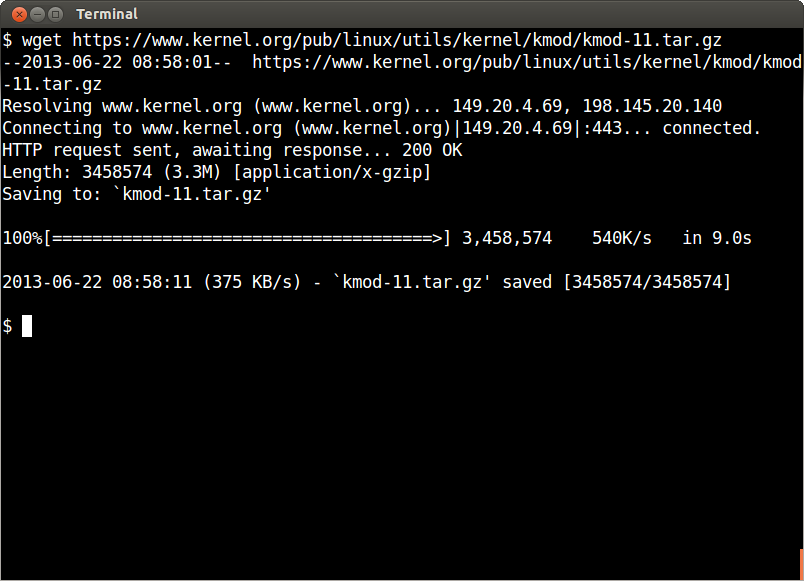
\includegraphics{./pictures/1-1-wget.png}
\caption{wget下载源码包}
\end{figure}

\subsubsection{tar解压源码包}

{\begin{shaded}\begin{verbatim}
$ tar zxf kmod-11.tar.gz 
$ cd kmod-11
$ ls
aclocal.m4   configure     libkmod      Makefile.in  README     tools
build-aux    configure.ac  m4           man          testsuite
config.h.in  COPYING       Makefile.am  NEWS         TODO
$ 
\end{verbatim}\end{shaded}}
\begin{figure}[htbp]
\centering
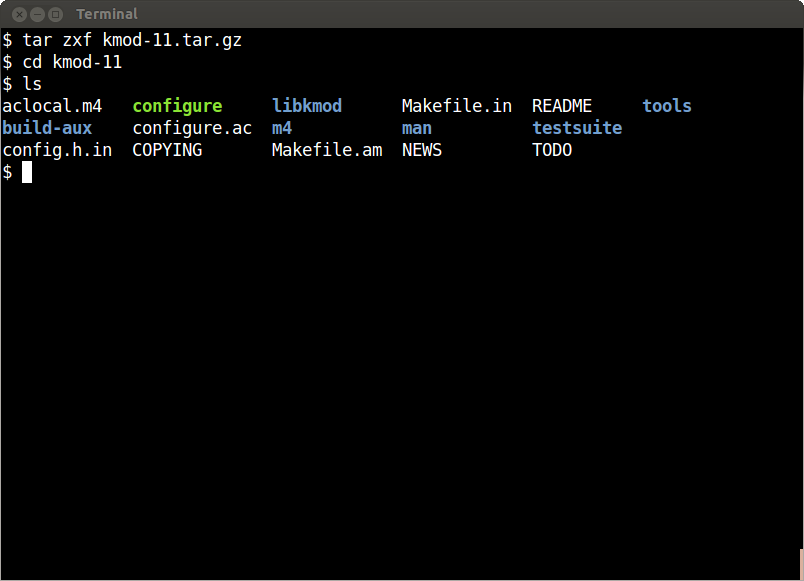
\includegraphics{./pictures/1-2-tar.png}
\caption{tar解压源码包}
\end{figure}

\subsubsection{configure 配置项目源码}

{\begin{shaded}\begin{verbatim}
$ ./configure CFLAGS="-g -O2" --prefix=/usr --sysconfdir=/etc --libdir=/usr/lib
checking for a BSD-compatible install... /usr/bin/install -c
checking whether build environment is sane... yes
checking for a thread-safe mkdir -p... /bin/mkdir -p
checking for gawk... no
checking for mawk... mawk
checking whether make sets $(MAKE)... yes
checking whether make supports nested variables... yes
checking how to create a pax tar archive... gnutar
checking for style of include used by make... GNU
checking for gcc... gcc
checking whether the C compiler works... yes
checking for C compiler default output file name... a.out
checking for suffix of executables... 
checking whether we are cross compiling... no
checking for suffix of object files... o
checking whether we are using the GNU C compiler... yes
checking whether gcc accepts -g... yes
checking for gcc option to accept ISO C89... none needed
checking dependency style of gcc... gcc3
...
kmod 11
======

prefix:         /usr
sysconfdir:     /etc
libdir:         /usr/lib
rootlibdir:     /usr/lib
includedir:     ${prefix}/include
bindir:         ${exec_prefix}/bin

compiler:       gcc -std=gnu99
cflags:          -pipe -DANOTHER_BRICK_IN_THE -Wall -W -Wextra -Wno-inline -Wvla -Wundef -Wformat=2 -Wlogical-op -Wsign-compare -Wformat-security -Wmissing-include-dirs -Wformat-nonliteral -Wold-style-definition -Wpointer-arith -Winit-self -Wdeclaration-after-statement -Wfloat-equal -Wmissing-prototypes -Wstrict-prototypes -Wredundant-decls -Wmissing-declarations -Wmissing-noreturn -Wshadow -Wendif-labels -Wstrict-aliasing=2 -Wwrite-strings -Wno-long-long -Wno-overlength-strings -Wno-unused-parameter -Wno-missing-field-initializers -Wno-unused-result -Wnested-externs -Wchar-subscripts -Wtype-limits -Wuninitialized -fno-common -fdiagnostics-show-option -fvisibility=hidden -ffunction-sections -fdata-sections -g -O2
ldflags:         -Wl,--as-needed -Wl,--gc-sections 

tools:          yes
logging:        yes
compression:        xz=no  zlib=no
debug:          no
doc:            no
man:            yes
\end{verbatim}\end{shaded}}
\begin{figure}[htbp]
\centering
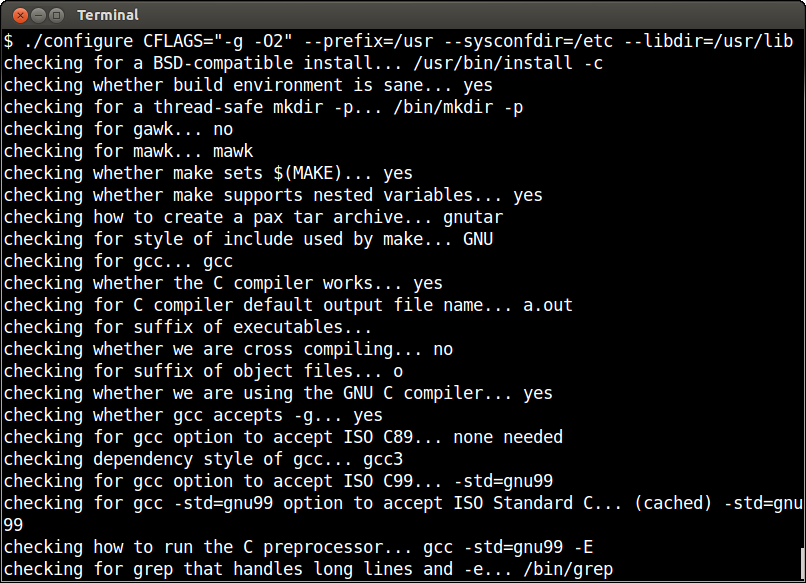
\includegraphics{./pictures/1-3-configure.png}
\caption{configure配置源码包}
\end{figure}

\subsubsection{编译项目源码}

{\begin{shaded}\begin{verbatim}
$ make
make --no-print-directory all-recursive
Making all in .
  CC       libkmod/libkmod.lo
  CC       libkmod/libkmod-list.lo
  CC       libkmod/libkmod-config.lo
  CC       libkmod/libkmod-index.lo
  CC       libkmod/libkmod-module.lo
  CC       libkmod/libkmod-file.lo
  CC       libkmod/libkmod-elf.lo
  CC       libkmod/libkmod-hash.lo
  CC       libkmod/libkmod-array.lo
  CC       libkmod/libkmod-util.lo
  CCLD     libkmod/libkmod-util.la
  CCLD     libkmod/libkmod.la
  CCLD     libkmod/libkmod-private.la
  CC       tools/kmod.o
  CC       tools/lsmod.o
  CC       tools/rmmod.o
  CC       tools/insmod.o
  CC       tools/modinfo.o
  CC       tools/modprobe.o
  CC       tools/depmod.o
  CC       tools/log.o
  CCLD     tools/kmod
  CCLD     tools/kmod-nolib
  GEN      tools/insmod
  GEN      tools/rmmod
  GEN      tools/lsmod
  GEN      tools/modprobe
  GEN      tools/modinfo
  GEN      tools/depmod
  GEN      libkmod/libkmod.pc
Making all in libkmod/docs
make[2]: Nothing to be done for `all'.
Making all in man
make[2]: Nothing to be done for `all'.
\end{verbatim}\end{shaded}}
\begin{figure}[htbp]
\centering
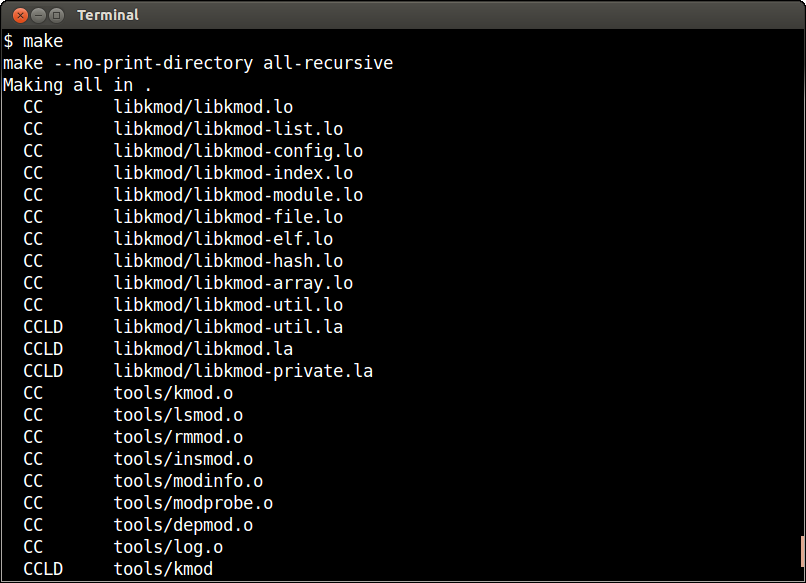
\includegraphics{./pictures/1-4-make.png}
\caption{make编译源码包}
\end{figure}

\subsubsection{测试生成命令}

{\begin{shaded}\begin{verbatim}
$ ./tools/insmod -h
Usage:
    insmod [options] filename [args]
Options:
    -V, --version     show version
    -h, --help        show this help
$ ./tools/rmmod -h
Usage:
    rmmod [options] modulename ...
Options:
    -f, --force       forces a module unload and may crash your
                  machine. This requires Forced Module Removal
                  option in your kernel. DANGEROUS
    -s, --syslog      print to syslog, not stderr
    -v, --verbose     enables more messages
    -V, --version     show version
    -h, --help        show this help
$ ./tools/lsmod -h
Usage: ./tools/lsmod
$ ./tools/modinfo -h
Usage:
    modinfo [options] filename [args]
Options:
    -a, --author                Print only 'author'
    -d, --description           Print only 'description'
    -l, --license               Print only 'license'
    -p, --parameters            Print only 'parm'
    -n, --filename              Print only 'filename'
    -0, --null                  Use \0 instead of \n
    -F, --field=FIELD           Print only provided FIELD
    -k, --set-version=VERSION   Use VERSION instead of `uname -r`
    -b, --basedir=DIR           Use DIR as filesystem root for /lib/modules
    -V, --version               Show version
    -h, --help                  Show this help
$ 
\end{verbatim}\end{shaded}}
\begin{figure}[htbp]
\centering
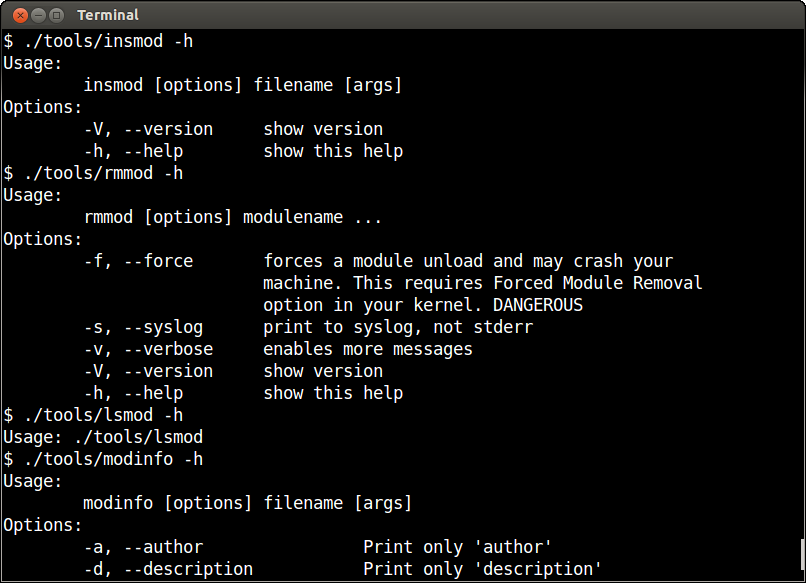
\includegraphics{./pictures/1-5-test.png}
\caption{测试生成命令}
\end{figure}

\subsection{项目Debug版运行调试图}

\subsubsection{配置时加上 --enable-debug, --enable-logging 参数}

{\begin{shaded}\begin{verbatim}
$ ./configure CFLAGS="-g -O2" --prefix=/usr --sysconfdir=/etc --libdir=/usr/lib --enable-debug --enable-logging
checking for a BSD-compatible install... /usr/bin/install -c
checking whether build environment is sane... yes
checking for a thread-safe mkdir -p... /bin/mkdir -p
checking for gawk... no
checking for mawk... mawk
checking whether make sets $(MAKE)... yes
checking whether make supports nested variables... yes
checking how to create a pax tar archive... gnutar
checking for style of include used by make... GNU
checking for gcc... gcc
checking whether the C compiler works... yes
checking for C compiler default output file name... a.out
checking for suffix of executables... 
checking whether we are cross compiling... no
checking for suffix of object files... o
checking whether we are using the GNU C compiler... yes
checking whether gcc accepts -g... yes
checking for gcc option to accept ISO C89... none needed
checking dependency style of gcc... gcc3
checking for gcc option to accept ISO C99... -std=gnu99
checking for gcc -std=gnu99 option to accept ISO Standard C... (cached) -std=gnu99
checking how to run the C preprocessor... gcc -std=gnu99 -E
checking for grep that handles long lines and -e... /bin/grep
checking for egrep... /bin/grep -E
checking for ANSI C header files... yes
checking for sys/types.h... yes
checking for sys/stat.h... yes
checking for stdlib.h... yes
checking for string.h... yes
checking for memory.h... yes
checking for strings.h... yes
checking for inttypes.h... yes
checking for stdint.h... yes
checking for unistd.h... yes
checking minix/config.h usability... no
checking minix/config.h presence... no
checking for minix/config.h... no
checking whether it is safe to define __EXTENSIONS__... yes
checking for special C compiler options needed for large files... no
checking for _FILE_OFFSET_BITS value needed for large files... 64
checking whether make supports nested variables... (cached) yes
checking build system type... i686-pc-linux-gnu
checking host system type... i686-pc-linux-gnu
checking how to print strings... printf
checking for a sed that does not truncate output... /bin/sed
checking for fgrep... /bin/grep -F
checking for ld used by gcc -std=gnu99... /usr/bin/ld
checking if the linker (/usr/bin/ld) is GNU ld... yes
checking for BSD- or MS-compatible name lister (nm)... /usr/bin/nm -B
checking the name lister (/usr/bin/nm -B) interface... BSD nm
checking whether ln -s works... yes
checking the maximum length of command line arguments... 1572864
checking whether the shell understands some XSI constructs... yes
checking whether the shell understands "+="... yes
checking how to convert i686-pc-linux-gnu file names to i686-pc-linux-gnu format... func_convert_file_noop
checking how to convert i686-pc-linux-gnu file names to toolchain format... func_convert_file_noop
checking for /usr/bin/ld option to reload object files... -r
checking for objdump... objdump
checking how to recognize dependent libraries... pass_all
checking for dlltool... no
checking how to associate runtime and link libraries... printf %s\n
checking for ar... ar
checking for archiver @FILE support... @
checking for strip... strip
checking for ranlib... ranlib
checking command to parse /usr/bin/nm -B output from gcc -std=gnu99 object... ok
checking for sysroot... no
checking for mt... mt
checking if mt is a manifest tool... no
checking for dlfcn.h... yes
checking for objdir... .libs
checking if gcc -std=gnu99 supports -fno-rtti -fno-exceptions... no
checking for gcc -std=gnu99 option to produce PIC... -fPIC -DPIC
checking if gcc -std=gnu99 PIC flag -fPIC -DPIC works... yes
checking if gcc -std=gnu99 static flag -static works... yes
checking if gcc -std=gnu99 supports -c -o file.o... yes
checking if gcc -std=gnu99 supports -c -o file.o... (cached) yes
checking whether the gcc -std=gnu99 linker (/usr/bin/ld) supports shared libraries... yes
checking whether -lc should be explicitly linked in... no
checking dynamic linker characteristics... GNU/Linux ld.so
checking how to hardcode library paths into programs... immediate
checking whether stripping libraries is possible... yes
checking if libtool supports shared libraries... yes
checking whether to build shared libraries... yes
checking whether to build static libraries... no
checking for gcc... (cached) gcc
checking whether we are using the GNU C compiler... (cached) yes
checking whether gcc accepts -g... (cached) yes
checking for gcc option to accept ISO C89... (cached) none needed
checking dependency style of gcc... (cached) gcc3
checking for gcc option to accept ISO C99... (cached) -std=gnu99
checking for typeof syntax and keyword spelling... typeof
checking whether gcc -std=gnu99 and cc understand -c and -o together... yes
checking whether gcc -std=gnu99 needs -traditional... no
checking whether byte ordering is bigendian... no
checking for a sed that does not truncate output... (cached) /bin/sed
checking for pkg-config... /usr/bin/pkg-config
checking pkg-config is at least version 0.9.0... yes
checking for __xstat... yes
checking for struct stat.st_mtim... yes
configure: Xz support not requested
configure: zlib support not requested
checking for xsltproc... /usr/bin/xsltproc
checking for gtkdoc-check... no
checking for gtkdoc-rebase... no
checking for gtkdoc-mkpdf... no
checking whether to build gtk-doc documentation... no
checking if gcc -std=gnu99 supports flag -pipe in envvar CFLAGS... yes
checking if gcc -std=gnu99 supports flag -DANOTHER_BRICK_IN_THE in envvar CFLAGS... yes
checking if gcc -std=gnu99 supports flag -Wall in envvar CFLAGS... yes
checking if gcc -std=gnu99 supports flag -W in envvar CFLAGS... yes
checking if gcc -std=gnu99 supports flag -Wextra in envvar CFLAGS... yes
checking if gcc -std=gnu99 supports flag -Wno-inline in envvar CFLAGS... yes
checking if gcc -std=gnu99 supports flag -Wvla in envvar CFLAGS... yes
checking if gcc -std=gnu99 supports flag -Wundef in envvar CFLAGS... yes
checking if gcc -std=gnu99 supports flag -Wformat=2 in envvar CFLAGS... yes
checking if gcc -std=gnu99 supports flag -Wlogical-op in envvar CFLAGS... yes
checking if gcc -std=gnu99 supports flag -Wsign-compare in envvar CFLAGS... yes
checking if gcc -std=gnu99 supports flag -Wformat-security in envvar CFLAGS... yes
checking if gcc -std=gnu99 supports flag -Wmissing-include-dirs in envvar CFLAGS... yes
checking if gcc -std=gnu99 supports flag -Wformat-nonliteral in envvar CFLAGS... yes
checking if gcc -std=gnu99 supports flag -Wold-style-definition in envvar CFLAGS... yes
checking if gcc -std=gnu99 supports flag -Wpointer-arith in envvar CFLAGS... yes
checking if gcc -std=gnu99 supports flag -Winit-self in envvar CFLAGS... yes
checking if gcc -std=gnu99 supports flag -Wdeclaration-after-statement in envvar CFLAGS... yes
checking if gcc -std=gnu99 supports flag -Wfloat-equal in envvar CFLAGS... yes
checking if gcc -std=gnu99 supports flag -Wmissing-prototypes in envvar CFLAGS... yes
checking if gcc -std=gnu99 supports flag -Wstrict-prototypes in envvar CFLAGS... yes
checking if gcc -std=gnu99 supports flag -Wredundant-decls in envvar CFLAGS... yes
checking if gcc -std=gnu99 supports flag -Wmissing-declarations in envvar CFLAGS... yes
checking if gcc -std=gnu99 supports flag -Wmissing-noreturn in envvar CFLAGS... yes
checking if gcc -std=gnu99 supports flag -Wshadow in envvar CFLAGS... yes
checking if gcc -std=gnu99 supports flag -Wendif-labels in envvar CFLAGS... yes
checking if gcc -std=gnu99 supports flag -Wstrict-aliasing=2 in envvar CFLAGS... yes
checking if gcc -std=gnu99 supports flag -Wwrite-strings in envvar CFLAGS... yes
checking if gcc -std=gnu99 supports flag -Wno-long-long in envvar CFLAGS... yes
checking if gcc -std=gnu99 supports flag -Wno-overlength-strings in envvar CFLAGS... yes
checking if gcc -std=gnu99 supports flag -Wno-unused-parameter in envvar CFLAGS... yes
checking if gcc -std=gnu99 supports flag -Wno-missing-field-initializers in envvar CFLAGS... yes
checking if gcc -std=gnu99 supports flag -Wno-unused-result in envvar CFLAGS... yes
checking if gcc -std=gnu99 supports flag -Wnested-externs in envvar CFLAGS... yes
checking if gcc -std=gnu99 supports flag -Wchar-subscripts in envvar CFLAGS... yes
checking if gcc -std=gnu99 supports flag -Wtype-limits in envvar CFLAGS... yes
checking if gcc -std=gnu99 supports flag -Wuninitialized in envvar CFLAGS... yes
checking if gcc -std=gnu99 supports flag -fno-common in envvar CFLAGS... yes
checking if gcc -std=gnu99 supports flag -fdiagnostics-show-option in envvar CFLAGS... yes
checking if gcc -std=gnu99 supports flag -fvisibility=hidden in envvar CFLAGS... yes
checking if gcc -std=gnu99 supports flag -ffunction-sections in envvar CFLAGS... yes
checking if gcc -std=gnu99 supports flag -fdata-sections in envvar CFLAGS... yes
checking if gcc -std=gnu99 supports flag -Wl,--as-needed in envvar LDFLAGS... yes
checking if gcc -std=gnu99 supports flag -Wl,--gc-sections in envvar LDFLAGS... yes
checking that generated files are newer than configure... done
configure: creating ./config.status
config.status: creating Makefile
config.status: creating man/Makefile
config.status: creating libkmod/docs/Makefile
config.status: creating libkmod/docs/version.xml
config.status: creating config.h
config.status: executing depfiles commands

config.status: executing libtool commands

    kmod 11
    ======

    prefix:         /usr
    sysconfdir:     /etc
    libdir:         /usr/lib
    rootlibdir:     /usr/lib
    includedir:     ${prefix}/include
    bindir:         ${exec_prefix}/bin

    compiler:       gcc -std=gnu99
    cflags:          -pipe -DANOTHER_BRICK_IN_THE -Wall -W -Wextra -Wno-inline -Wvla -Wundef -Wformat=2 -Wlogical-op -Wsign-compare -Wformat-security -Wmissing-include-dirs -Wformat-nonliteral -Wold-style-definition -Wpointer-arith -Winit-self -Wdeclaration-after-statement -Wfloat-equal -Wmissing-prototypes -Wstrict-prototypes -Wredundant-decls -Wmissing-declarations -Wmissing-noreturn -Wshadow -Wendif-labels -Wstrict-aliasing=2 -Wwrite-strings -Wno-long-long -Wno-overlength-strings -Wno-unused-parameter -Wno-missing-field-initializers -Wno-unused-result -Wnested-externs -Wchar-subscripts -Wtype-limits -Wuninitialized -fno-common -fdiagnostics-show-option -fvisibility=hidden -ffunction-sections -fdata-sections -g -O2
    ldflags:         -Wl,--as-needed -Wl,--gc-sections 

    tools:          yes
    logging:        yes
    compression:        xz=no  zlib=no
    debug:          yes
    doc:            no
    man:            yes
\end{verbatim}\end{shaded}}
\begin{figure}[htbp]
\centering
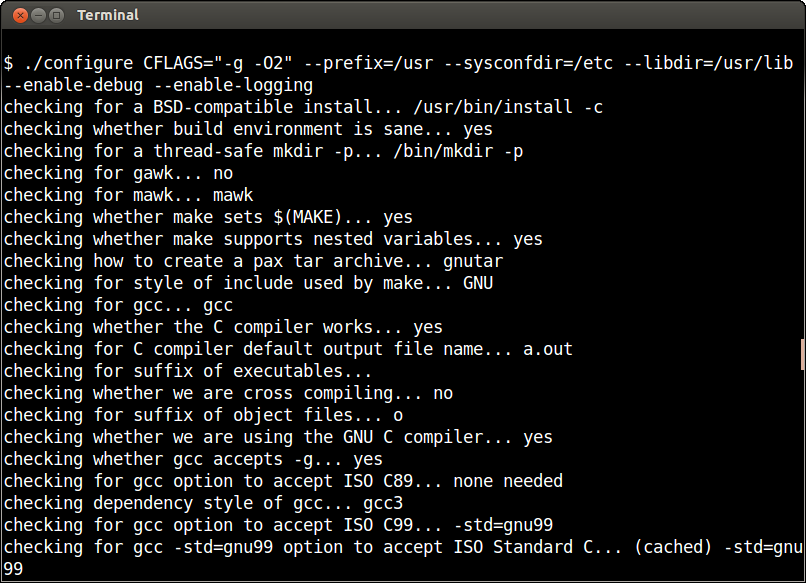
\includegraphics{./pictures/2-1-configure.png}
\caption{配置时加上调试参数}
\end{figure}

\subsubsection{make clean \&\& make 重新编译}

{\begin{shaded}\begin{verbatim}
$ make clean && make
Making clean in .
 rm -f tools/kmod
test -z "testsuite/uname.la testsuite/path.la testsuite/init_module.la testsuite/delete_module.la testsuite/libtestsuite.la" || rm -f testsuite/uname.la testsuite/path.la testsuite/init_module.la testsuite/delete_module.la testsuite/libtestsuite.la
rm -f testsuite/so_locations
 rm -f testsuite/test-init testsuite/test-testsuite testsuite/test-loaded testsuite/test-modinfo testsuite/test-alias testsuite/test-new-module testsuite/test-modprobe testsuite/test-blacklist testsuite/test-dependencies testsuite/test-depmod
test -z "libkmod/libkmod.pc" || rm -f libkmod/libkmod.pc
test -z "libkmod/libkmod.la" || rm -f libkmod/libkmod.la
rm -f libkmod/so_locations
rm -rf .libs _libs
rm -rf libkmod/.libs libkmod/_libs
rm -rf testsuite/.libs testsuite/_libs
rm -rf tools/.libs tools/_libs
test -z "libkmod/libkmod-util.la libkmod/libkmod-private.la" || rm -f libkmod/libkmod-util.la libkmod/libkmod-private.la
rm -f libkmod/so_locations
 rm -f tools/kmod-nolib
rm -f *.o
rm -f libkmod/*.o
rm -f libkmod/*.lo
rm -f testsuite/*.o
rm -f testsuite/*.lo
rm -f tools/*.o
rm -f *.lo
Making clean in libkmod/docs
test -z "" || rm -f 
rm -rf .libs _libs
rm -f *.lo
Making clean in man
test -z "depmod.d.5 modprobe.d.5 modules.dep.5 depmod.8 insmod.8 lsmod.8 rmmod.8 modprobe.8 modinfo.8 modules.dep.bin.5" || rm -f depmod.d.5 modprobe.d.5 modules.dep.5 depmod.8 insmod.8 lsmod.8 rmmod.8 modprobe.8 modinfo.8 modules.dep.bin.5
rm -rf .libs _libs
rm -f *.lo
make --no-print-directory all-recursive
Making all in .
  CC       libkmod/libkmod.lo
  CC       libkmod/libkmod-list.lo
  CC       libkmod/libkmod-config.lo
  CC       libkmod/libkmod-index.lo
  CC       libkmod/libkmod-module.lo
  CC       libkmod/libkmod-file.lo
  CC       libkmod/libkmod-elf.lo
  CC       libkmod/libkmod-hash.lo
  CC       libkmod/libkmod-array.lo
  CC       libkmod/libkmod-util.lo
  CCLD     libkmod/libkmod-util.la
  CCLD     libkmod/libkmod.la
  CCLD     libkmod/libkmod-private.la
  CC       tools/kmod.o
  CC       tools/lsmod.o
  CC       tools/rmmod.o
  CC       tools/insmod.o
  CC       tools/modinfo.o
  CC       tools/modprobe.o
  CC       tools/depmod.o
  CC       tools/log.o
  CCLD     tools/kmod
  CCLD     tools/kmod-nolib
  GEN      libkmod/libkmod.pc
Making all in libkmod/docs
make[2]: Nothing to be done for `all'.
Making all in man
  GEN      depmod.d.5
  GEN      modprobe.d.5
  GEN      modules.dep.5
  GEN      depmod.8
  GEN      insmod.8
  GEN      lsmod.8
  GEN      rmmod.8
  GEN      modprobe.8
  GEN      modinfo.8
$ 
\end{verbatim}\end{shaded}}
\begin{figure}[htbp]
\centering
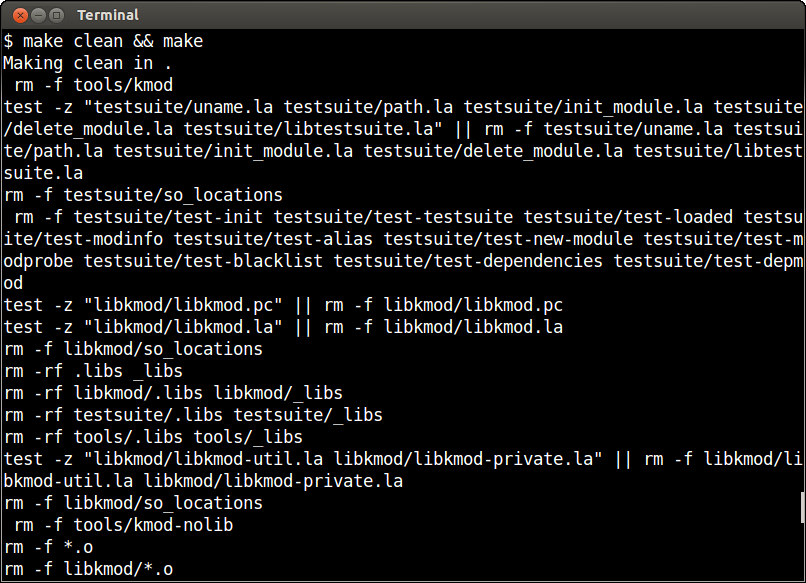
\includegraphics{./pictures/2-2-make.png}
\caption{make重新编译}
\end{figure}

\subsubsection{设置日志优先级 KMOD\_LOG=7}

{\begin{shaded}\begin{verbatim}
$ sudo KMOD_LOG=7 ./tools/insmod ../hello-module/hello.ko
libkmod: INFO libkmod/libkmod.c:275 kmod_new: ctx 0x9243008 created
libkmod: DEBUG libkmod/libkmod.c:276 kmod_new: log_priority=7
libkmod: DEBUG libkmod/libkmod.c:389 kmod_pool_get_module: get module name='hello' found=(nil)
libkmod: DEBUG libkmod/libkmod.c:389 kmod_pool_get_module: get module name='hello' found=(nil)
libkmod: DEBUG libkmod/libkmod.c:397 kmod_pool_add_module: add 0x9243088 key='hello'
libkmod: DEBUG libkmod/libkmod-module.c:718 kmod_module_get_path: name='hello' path='/home/akaedu/Github/test-kmod-11/kmod-11/../hello-module/hello.ko'
libkmod: DEBUG libkmod/libkmod-module.c:440 kmod_module_unref: kmod_module 0x9243088 released
libkmod: DEBUG libkmod/libkmod.c:405 kmod_pool_del_module: del 0x9243088 key='hello'
libkmod: INFO libkmod/libkmod.c:318 kmod_unref: context 0x9243008 released
$ 
\end{verbatim}\end{shaded}}
\begin{figure}[htbp]
\centering
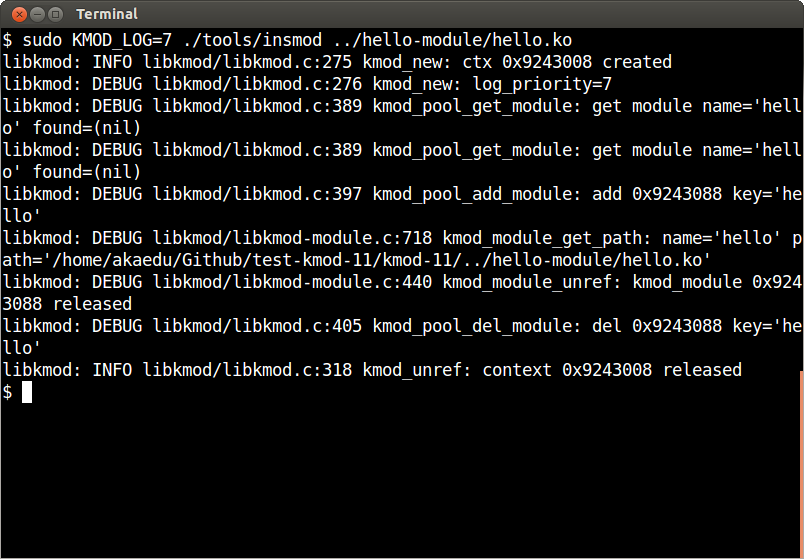
\includegraphics{./pictures/2-3-insmod.png}
\caption{设置 KMOD\_LOG=7 模式下插入模块}
\end{figure}

\subsubsection{卸载模块以便进行下一次插入}

{\begin{shaded}\begin{verbatim}
$ sudo KMOD_LOG=7 ./tools/rmmod ../hello-module/hello.ko
libkmod: INFO libkmod/libkmod.c:275 kmod_new: ctx 0x9584008 created
libkmod: DEBUG libkmod/libkmod.c:276 kmod_new: log_priority=7
$ 
\end{verbatim}\end{shaded}}
\subsubsection{设置日志优先级 KMOD\_LOG=6}

{\begin{shaded}\begin{verbatim}
$ sudo KMOD_LOG=6 ./tools/insmod ../hello-module/hello.ko
libkmod: INFO libkmod/libkmod.c:275 kmod_new: ctx 0x9c46008 created
libkmod: INFO libkmod/libkmod.c:318 kmod_unref: context 0x9c46008 released
$ 

$ sudo KMOD_LOG=6 ./tools/rmmod ../hello-module/hello.ko
libkmod: INFO libkmod/libkmod.c:275 kmod_new: ctx 0x9584008 created
libkmod: DEBUG libkmod/libkmod.c:276 kmod_new: log_priority=7
$ 
\end{verbatim}\end{shaded}}
\begin{figure}[htbp]
\centering
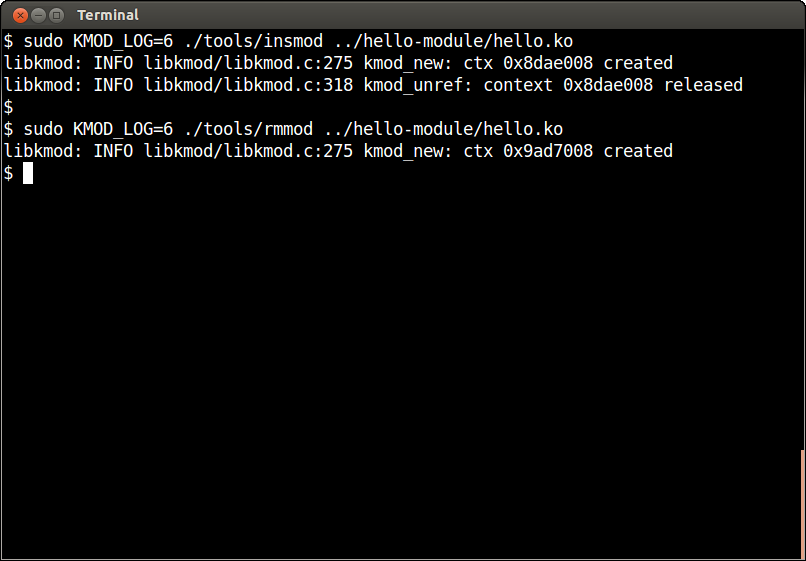
\includegraphics{./pictures/2-4-insmod2.png}
\caption{设置 KMOD\_LOG=6 模式下插入模块}
\end{figure}

\subsection{源码修改运行调试图}

\subsubsection{修改 modprobe.c 源码}

\subsubsection{修改 kmod\_module\_parse\_depline 函数}

{\begin{shaded}\begin{verbatim}
$ vi kmod-11/libkmod/libkmod-module.c +120
120 int kmod_module_parse_depline(struct kmod_module *mod, char *line)
121 {
122         struct kmod_ctx *ctx = mod->ctx;
123         struct kmod_list *list = NULL;
124         const char *dirname;
125         char buf[PATH_MAX];
126         char *p, *saveptr;
127         int err = 0, n = 0;
128         size_t dirnamelen;
129 
130         printf("<mydebug> line = %s\n", line);
131 
132         if (mod->init.dep)
133                 return mod->n_dep;
134         assert(mod->dep == NULL);
135         mod->init.dep = true;
136 
137         p = strchr(line, ':');
138         if (p == NULL)
139                 return 0;
140 
\end{verbatim}\end{shaded}}
\begin{figure}[htbp]
\centering
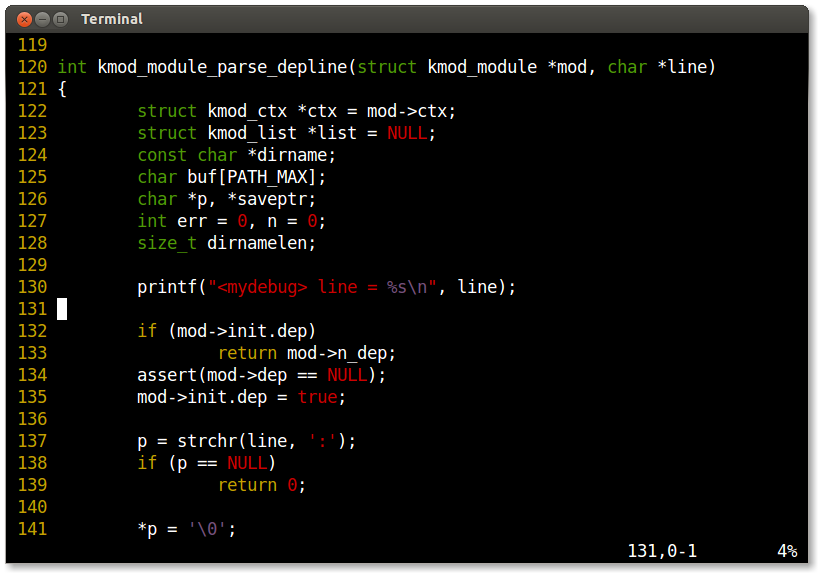
\includegraphics{./pictures/3-1-depline.png}
\caption{插入130行的打印 line 的语句}
\end{figure}

\subsubsection{重新编译生成新的 modprobe}

{\begin{shaded}\begin{verbatim}
$ make -C kmod-11/
make: Entering directory `/home/akaedu/Github/test-kmod-11/kmod-11'
make --no-print-directory all-recursive
Making all in .
  CC       libkmod/libkmod-module.lo
  CCLD     libkmod/libkmod.la
  CCLD     libkmod/libkmod-private.la
  CCLD     tools/kmod
  CCLD     tools/kmod-nolib
Making all in libkmod/docs
make[2]: Nothing to be done for `all'.
Making all in man
make[2]: Nothing to be done for `all'.
make: Leaving directory `/home/akaedu/Github/test-kmod-11/kmod-11'
$ 
\end{verbatim}\end{shaded}}
\begin{figure}[htbp]
\centering
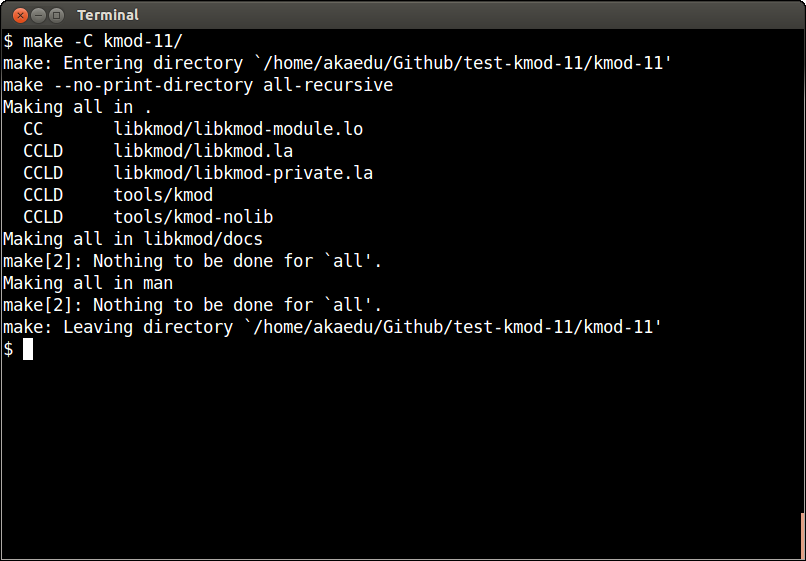
\includegraphics{./pictures/3-2-make.png}
\caption{make编译成功,增量编译了libkmod-module模块}
\end{figure}

\subsubsection{运行 modprobe nfs}

{\begin{shaded}\begin{verbatim}
$ ./kmod-11/tools/modprobe nfs
<mydebug> line = kernel/fs/nfs/nfs.ko: kernel/fs/nfs_common/nfs_acl.ko kernel/net/sunrpc/auth_gss/auth_rpcgss.ko kernel/fs/fscache/fscache.ko kernel/fs/lockd/lockd.ko kernel/net/sunrpc/sunrpc.ko

$ lsmod | grep nfs
nfsd                  229850  13 
nfs                   307376  0 
nfs_acl                12771  2 nfsd,nfs
auth_rpcgss            39597  2 nfsd,nfs
fscache                50642  1 nfs
lockd                  78804  2 nfsd,nfs
sunrpc                205647  19 nfsd,nfs,nfs_acl,auth_rpcgss,lockd
$ 
\end{verbatim}\end{shaded}}
\begin{figure}[htbp]
\centering
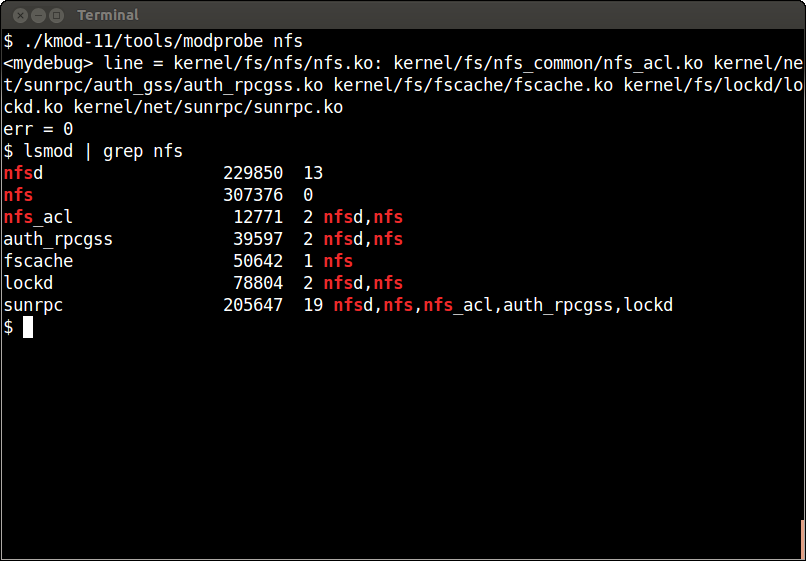
\includegraphics{./pictures/3-3-modprobe.png}
\caption{运行 modprobe nfs 完成插入}
\end{figure}

\subsubsection{插入167行打印语句}

{\begin{shaded}\begin{verbatim}
$ vi kmod-11/libkmod/libkmod-module.c +161
161         p++;
162         for (p = strtok_r(p, " \t", &saveptr); p != NULL;
163                                         p = strtok_r(NULL, " \t", &saveptr)     ) {
164                 struct kmod_module *depmod;
165                 const char *path;
166 
167                 printf("<mydebug> p = %s\n", p);
168                 path = path_join(p, dirnamelen, buf);
169                 if (path == NULL) {
170                         ERR(ctx, "could not join path '%s' and '%s'.\n",
171                             dirname, p);
172                         goto fail;
173                 }
\end{verbatim}\end{shaded}}
\begin{figure}[htbp]
\centering
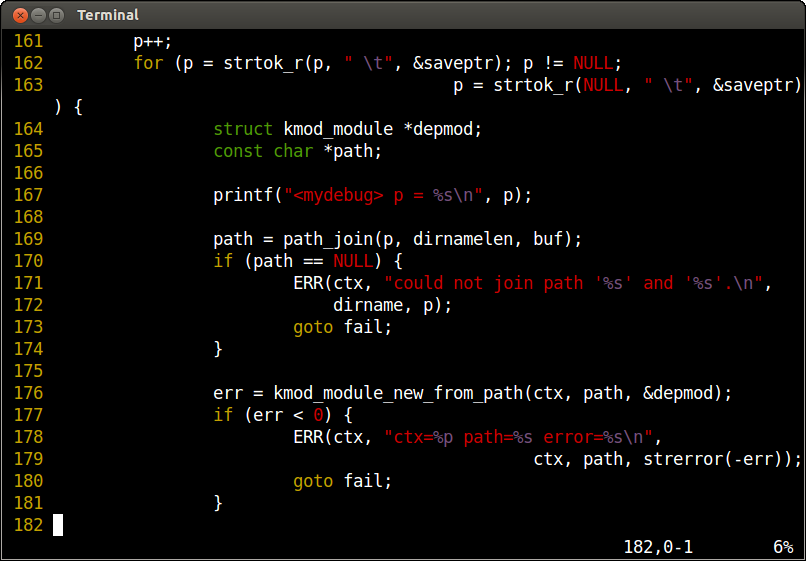
\includegraphics{./pictures/3-4-print-p.png}
\caption{插入打印每个模块名称的调试代码}
\end{figure}

\subsubsection{重新编译生成新的 modprobe}

{\begin{shaded}\begin{verbatim}
$ make -C kmod-11/
make: Entering directory `/home/akaedu/Github/test-kmod-11/kmod-11'
make --no-print-directory all-recursive
Making all in .
  CC       libkmod/libkmod-module.lo
  CCLD     libkmod/libkmod.la
  CCLD     libkmod/libkmod-private.la
  CCLD     tools/kmod
  CCLD     tools/kmod-nolib
Making all in libkmod/docs
make[2]: Nothing to be done for `all'.
Making all in man
make[2]: Nothing to be done for `all'.
make: Leaving directory `/home/akaedu/Github/test-kmod-11/kmod-11'
$ 
\end{verbatim}\end{shaded}}
\subsubsection{运行 modprobe nfs}

{\begin{shaded}\begin{verbatim}
$ ./kmod-11/tools/modprobe nfs
<mydebug> line = kernel/fs/nfs/nfs.ko: kernel/fs/nfs_common/nfs_acl.ko kernel/net/sunrpc/auth_gss/auth_rpcgss.ko kernel/fs/fscache/fscache.ko kernel/fs/lockd/lockd.ko kernel/net/sunrpc/sunrpc.ko
<mydebug> p = kernel/fs/nfs_common/nfs_acl.ko
<mydebug> p = kernel/net/sunrpc/auth_gss/auth_rpcgss.ko
<mydebug> p = kernel/fs/fscache/fscache.ko
<mydebug> p = kernel/fs/lockd/lockd.ko
<mydebug> p = kernel/net/sunrpc/sunrpc.ko
\end{verbatim}\end{shaded}}
\begin{figure}[htbp]
\centering
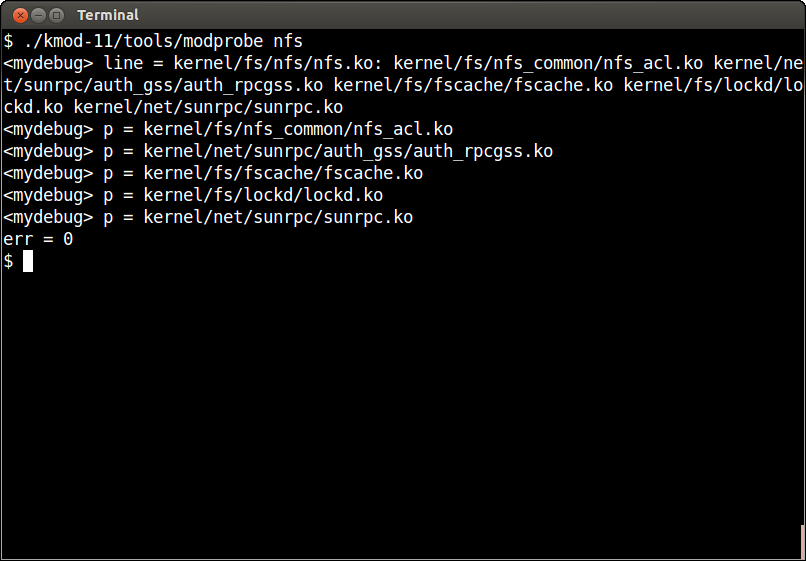
\includegraphics{./pictures/3-5-print-p-output.png}
\caption{调试代码输出详细调试信息}
\end{figure}

\end{document}
